\chapter{Results}
\label{chap:results}

All results in this chapter come from a single run per arm over all 101 tasks in manifest order. Accuracy pools all test cases (as in the official script); the learning curve averages per-task accuracy, so its end points differ slightly.

\section{Main Comparison}
\Cref{tab:main} compares the three arms on the same tasks.

\begin{table}[ht]
\centering
\caption{Results on all 101 tasks (single run, manifest order). Accuracy in \%. Appearance is averaged over tasks with an appearance grade.}
\label{tab:main}
\begin{tabular}{lccc}
\toprule
Arm & Accuracy & Appearance & Zero-score tasks \\
\midrule
No Memory & 28.5 & 3.25 & 30 \\
Long Memory v4 & 30.9 & 3.21 & 20 \\
Long Memory v7 & \textbf{40.0} & 3.21 & \textbf{13} \\
\bottomrule
\end{tabular}
\end{table}

Per task, v7 beats No Memory on 54 tasks, loses on 24 and ties on 23; the mean paired difference in per-task accuracy is $+11.5$ points (95\% bootstrap \gls{ci} $[6.0, 16.9]$). Against v4 the difference is $+8.9$ points ($[2.9, 15.1]$; 53 wins, 29 losses, 19 ties).

\section{Learning Curve}
\Cref{fig:curve} plots cumulative and rolling accuracy in execution order. v4 and v7 are similar on the first 30 tasks (39.3\% and 39.0\%, versus 26.0\% for No Memory), when the code pool has few active entries. On the remaining 71 tasks v4 falls below No Memory (27.8\% vs 29.5\%, 19 zero-score tasks each), while v7 keeps its level (40.4\%, 9 zero-score tasks). On the last 35 tasks the gap is 38.3\% (v7) vs 26.0\% (No Memory) vs 23.2\% (v4).

\begin{figure}[ht]
\centering
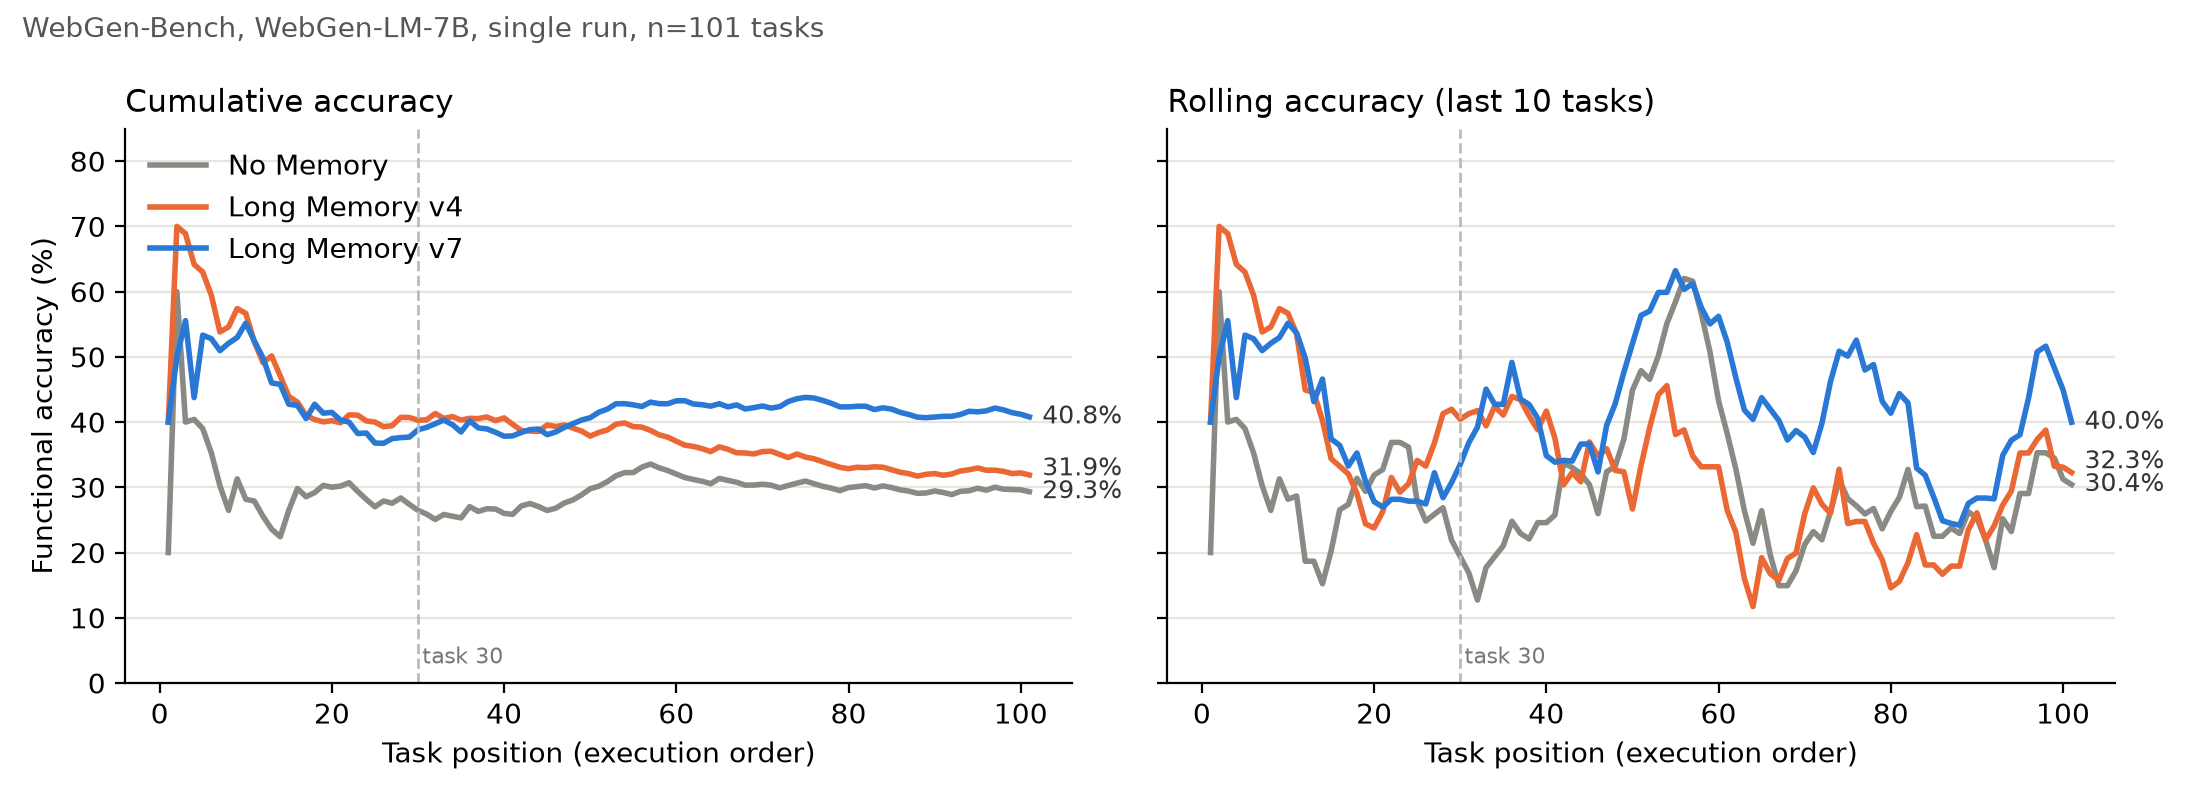
\includegraphics[width=\textwidth]{figures/learning_curve_v4_v7.png}
\caption{Cumulative and rolling-10 accuracy by execution order for No Memory, v4 and v7.}
\label{fig:curve}
\end{figure}

\Cref{fig:gap} shows the same data as a paired gap to No Memory. Both memories lead early; between tasks 40 and 60 v4 falls up to 27 points below No Memory while v7 stays near or above zero, and from task 60 onwards v7 stays clearly positive.

\begin{figure}[ht]
\centering
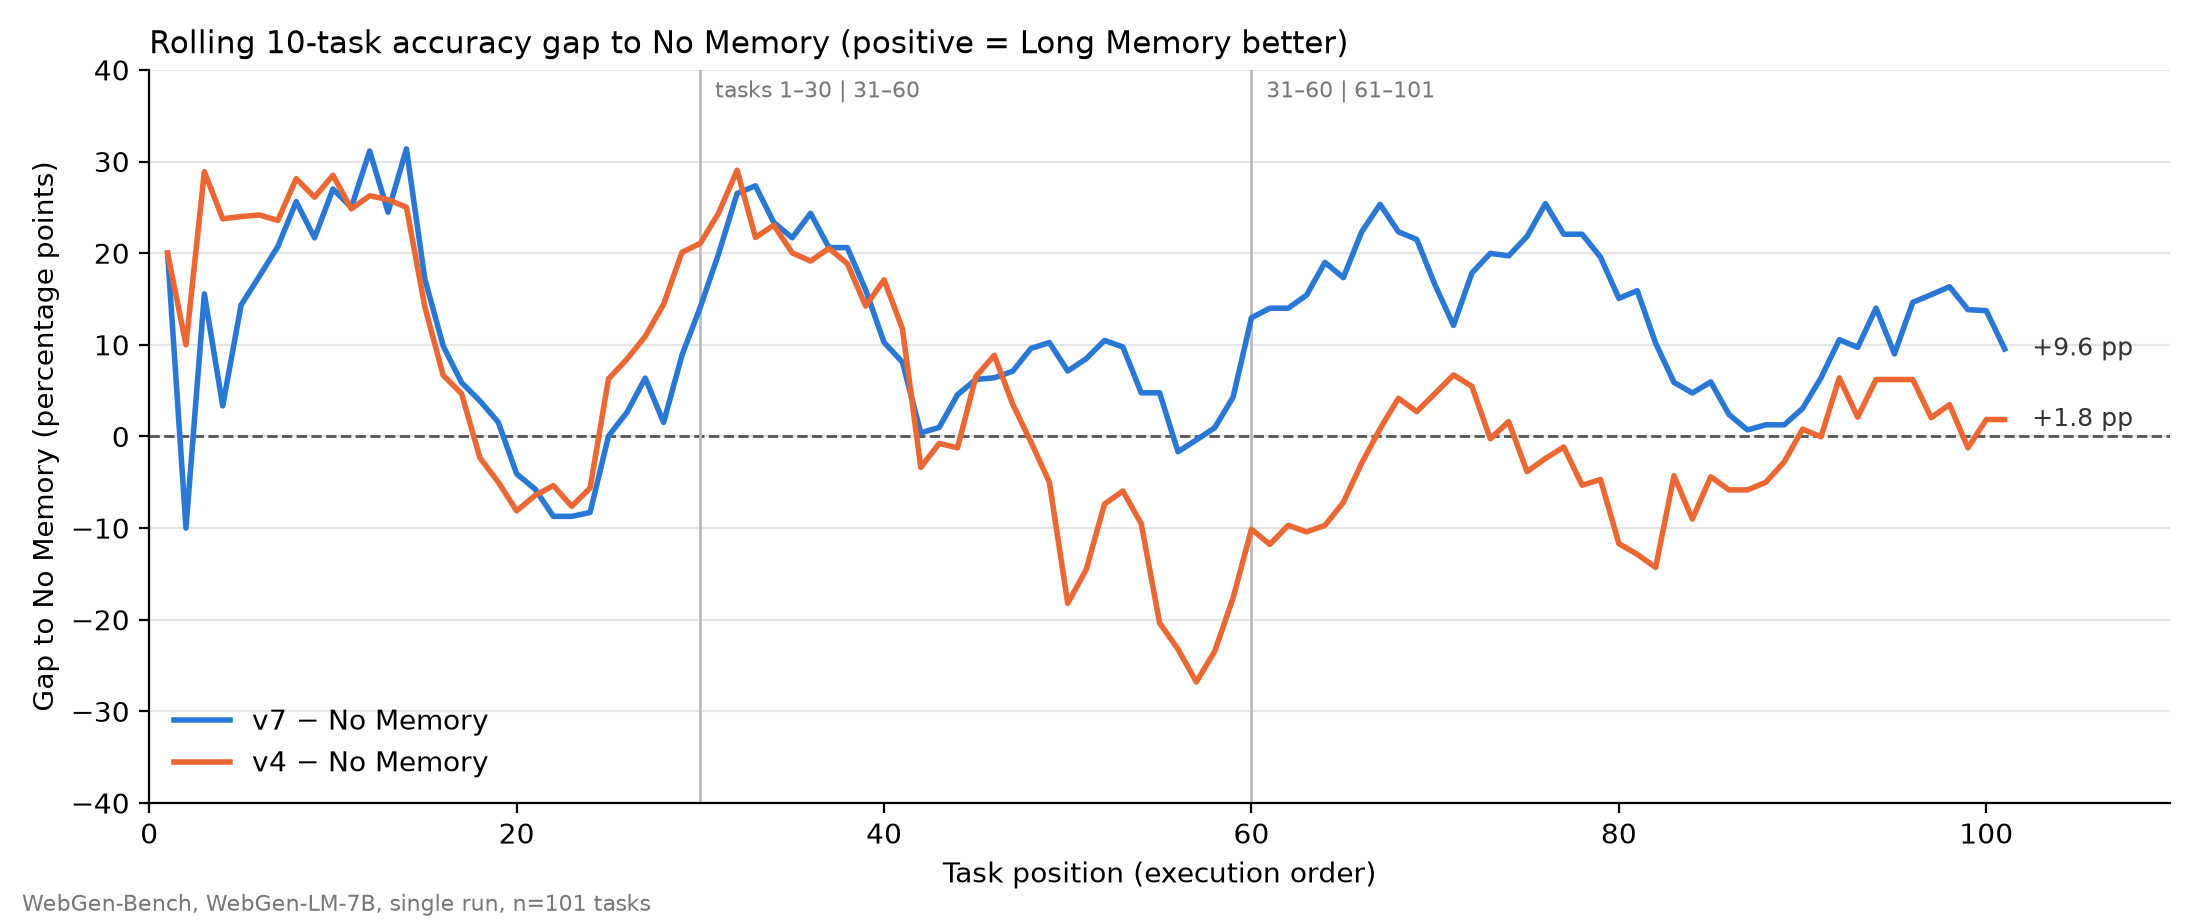
\includegraphics[width=\textwidth]{figures/gap_curve_v4_v7.png}
\caption{Rolling 10-task mean of the per-task accuracy gap to No Memory, by execution order. Positive values mean Long Memory is better.}
\label{fig:gap}
\end{figure}

\section{Why v4 Declines and v7 Improves}
\Cref{tab:prompt} counts what reached the generator's prompt, and \Cref{tab:codeerr} counts code problems in the generated sites, obtained by compiling every site with \texttt{@vue/compiler-sfc} 3.5.43. A lesson is counted as \emph{without a code construct} if it contains none of \texttt{@click}, \texttt{v-if}, \texttt{v-for}, \texttt{v-model}, \texttt{ref}, an \texttt{import} or inline code. In v4 such lessons appear in most tasks throughout and a separate ``General notes'' block becomes more frequent over time, while nothing addresses blank pages. In v7 these lessons are rarer and the code pool supplies a fragment in almost every task after it activates.

\begin{table}[ht]
\centering
\caption{Prompt content by segment (tasks 1--30 / 31--60 / 61--101).}
\label{tab:prompt}
\begin{tabular}{lcc}
\toprule
Prompt content & v4 & v7 \\
\midrule
Tasks with a lesson without a code construct & 23 / 25 / 28 & 12 / 4 / 11 \\
Tasks with a ``General notes'' block & 13 / 16 / 27 & 3 / 0 / 8 \\
Tasks with a code-pool fragment & 0 / 0 / 0 & 25 / 30 / 41 \\
Lessons attached to checklist items & 56 / 53 / 81 & 32 / 16 / 41 \\
\quad of which without a code construct (all tasks) & 102 of 190 & 31 of 89 \\
\bottomrule
\end{tabular}
\end{table}

\begin{table}[ht]
\centering
\small
\caption{Generated sites with code problems (number of tasks; 1--30 / 31--60 / 61--101, total in brackets).}
\label{tab:codeerr}
\begin{tabular}{lccc}
\toprule
Problem & No Memory & v4 & v7 \\
\midrule
Whole-site break\textsuperscript{a} & 11 / 5 / 10 (26) & 2 / 5 / 12 (19) & 4 / 1 / 3 (\textbf{8}) \\
Missing Vue import on a page & 7 / 7 / 9 (23) & 14 / 10 / 7 (31) & 12 / 4 / 6 (22) \\
\bottomrule
\multicolumn{4}{l}{\footnotesize \textsuperscript{a} An undeclared package import or a Vue compile error.}
\end{tabular}
\end{table}

These counts are correlational. Disentangling the contribution of each component requires the ablations in \Cref{sec:ablation}.

\section{Error Analysis}
Whole-site breaks fall from 26 tasks (No Memory) to 8 (v7), whereas pages with a missing Vue import are about as frequent as without memory (23 vs 22): the code pool prevents the error that blanks the whole site more reliably than the per-page one, which remains a basic error of the 7B generator. Counted per file, 27 of 592 generated Vue components in v7 (4.6\%) call a Vue function without importing it, against 27 of 586 (4.6\%) for No Memory. The omission occurs in \texttt{App.vue} and in child components alike, and is unrelated to whether a component uses \texttt{defineProps}/\texttt{defineEmits}; in the same file other imports are usually correct. It behaves like a random slip at a roughly constant per-file rate rather than a misconception, so a site with more components is more likely to contain one.

\paragraph{An attempted fix.} We tested a variant (v8) that rebuilds the code-pool example whenever the set of frequently missed functions changes, so that it shows both \texttt{ref} and \texttt{computed} (the v7 example was built at task 6 and only ever showed \texttt{ref}). Replacing only the code-pool section of the original v7 prompts, missing imports disappeared in one of four affected tasks and remained in the other three; two high-scoring regression tasks were unaffected. Because a random slip is not corrected by an example, and repairing generated code after generation is not allowed under the official protocol, we kept v7 as the final version and report this error rate as a limitation of the generator. Ten of v7's 13 zero-score tasks are also zero for No Memory, suggesting that most remaining failures are genuinely hard tasks for this generator.

Two v7 tasks returned the unmodified scaffold. A local diagnosis traced both to an example that was a complete \texttt{App.vue} file from another site; reducing it to a verified fragment restored real output on one task. This fix is not part of the frozen v7 run.

\paragraph{Appearance.} Restricted to the 68 tasks where both No Memory and v7 produced a working site with an appearance grade, the mean appearance score is 3.25 for No Memory and 3.22 for v7. The improvement is therefore functional; memory makes more sites work but does not make working sites look better.

\section{Ablation: Checklist Only}
\label{sec:ablation}
To separate the effect of requirement decomposition from that of memory, we run v7 with memory writes disabled, on the same task order. \todo{Fill in: Checklist-only accuracy / appearance / zero-score; contribution of checklist vs memory.}

\section{Robustness to Task Order}
\label{sec:order-design}
With memory, the order of tasks determines which experience is available, so a single order is not sufficient evidence. We therefore run Long Memory from an empty memory four times, each over all 101 tasks:
\begin{enumerate}
  \item the manifest (domain-block) order;
  \item a stratified shuffle with seed 11;
  \item a stratified shuffle with seed 29;
  \item a cross-domain interleaved order.
\end{enumerate}
In each order, Long Memory and No Memory are run as pairs on each task, alternating which arm runs first in an ABBA pattern, so that drift in infrastructure or evaluator load affects both arms equally. Results are reported per order as task-level paired differences with bootstrap \glspl{ci}, and by domain and position.

\begin{table}[ht]
\centering
\caption{Task-order experiments. \todo{Fill in when complete.}}
\label{tab:order}
\begin{tabular}{lcccc}
\toprule
Order & NM acc. & LM acc. & Paired diff. (95\% \gls{ci}) & Zero-score NM / LM \\
\midrule
Manifest & -- & -- & -- & -- \\
Shuffle (seed 11) & -- & -- & -- & -- \\
Shuffle (seed 29) & -- & -- & -- & -- \\
Interleaved & -- & -- & -- & -- \\
\bottomrule
\end{tabular}
\end{table}

\todo{Interpretation: stable gain in all orders (general benefit), gain only in domain blocks (curriculum effect), or worse when interleaved (cross-domain retrieval bottleneck).}
